\subsection{Quản lí source code}
 % phần này ghi cách làm việc với source code của nhóm: quy trình làm việc nhóm chuẩn: tạo nhánh -> làm -> đẩy code -> tạo merge req -> review -> merge. 

Ở đồ án này, nhóm sử dụng GitHub để quản lý sourcce code và tương tác với các thành viên khác. Nhằm tạo sự thống nhất, tiện lợi và hiệu quả trong quá trình làm việc nhóm với source code, chúng ta sẽ sử dụng \textbf{GitHub flow branching strategy } được đề xuất bởi chính GitHub. \\
% Nhớ tạo ref cho cái này https://docs.github.com/en/get-started/quickstart/github-flow

GitHub flow branching strategy là một quy trình làm việc tương đối đơn giản cho phép các nhóm nhỏ hoặc các ứng dụng/sản phẩm web không yêu cầu hỗ trợ nhiều phiên bản để nhanh chóng hoàn thành công việc của họ. \\

Trong GitHub flow, nhánh chính chứa mã nguồn đã sẵn sàng cho sản xuất. Các nhánh khác, được gọi là nhánh tính năng, nên chứa công việc về các tính năng mới và sửa lỗi, và sẽ được hợp nhất trở lại nhánh chính khi công việc hoàn thành và được đánh giá đúng cách. 
\subsubsection{GitHub Flow Best Practices}
Khi làm việc với chiến lược GitHub flow branching, có sáu nguyên tắc cần nên tuân thủ để đảm bảo duy trì mã nguồn tốt:
\begin{itemize}
    \item Mọi mã nguồn trong nhánh main nên có thể triển khai.
    \item Tạo các nhánh mới có tên mô tả rõ ràng từ nhánh chính để thực hiện công việc mới, chẳng hạn như features/add-new-payment-types.
    \item Commit công việc mới vào các nhánh local và thường xuyên push công việc lên remote.
    \item Để yêu cầu phản hồi hoặc sự giúp đỡ, hoặc khi nghĩ rằng công việc của mình đã sẵn sàng để hợp nhất vào nhánh chính, mở một pull request.
    \item Sau khi công việc hoặc tính năng của bạn đã được xem xét và chấp nhận, nó có thể được hợp nhất vào nhánh main.
    \item Sau khi công việc đã được hợp nhất vào nhánh main, nó nên được triển khai ngay lập tức.
\end{itemize}

\subsubsection{GitHub Flow: Lợi ích và nhược điểm}
\begin{figure}[H]
    \centering
    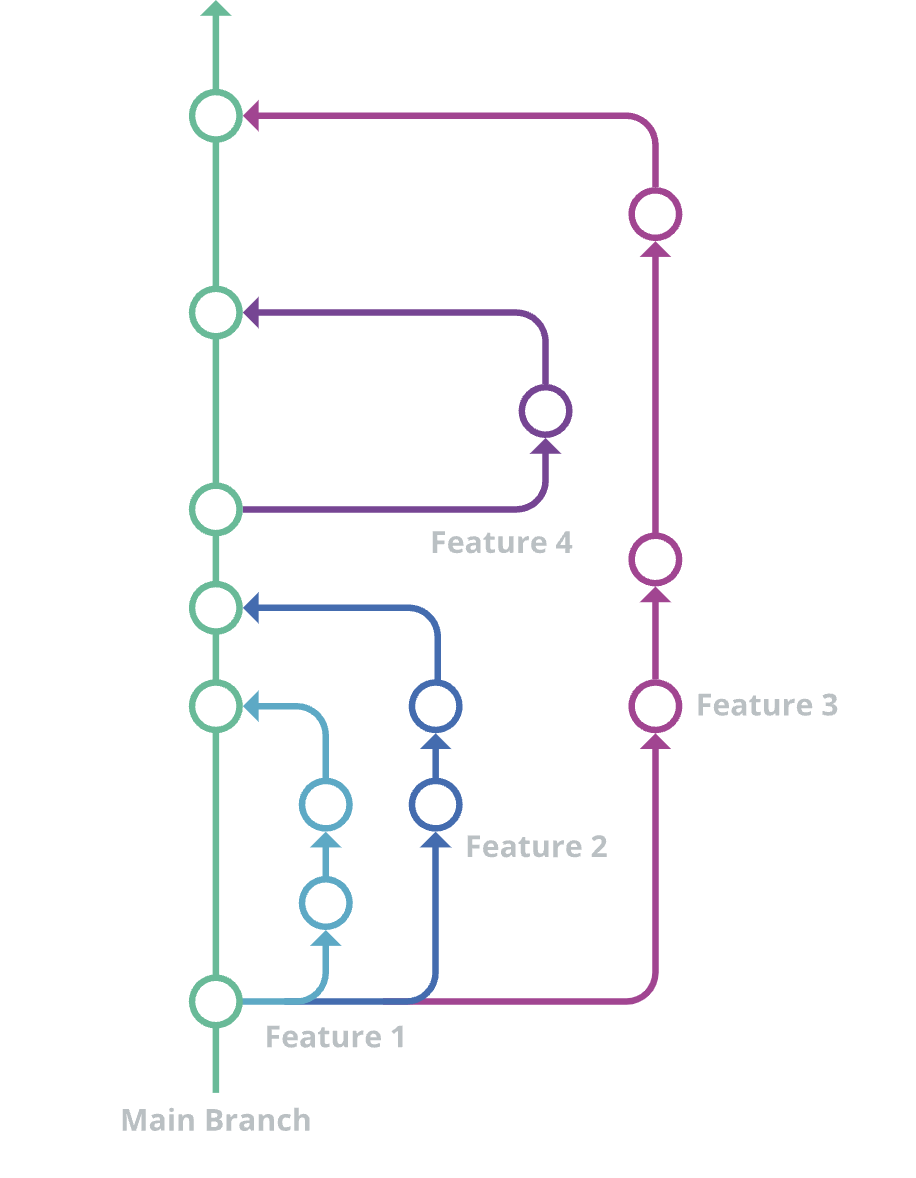
\includegraphics[width=8cm]{Images/githubflow.png}
    \vspace{0.5cm}
    \caption{Mô phỏng các branch trong 1 GitHub flow}
\end{figure}
\begin{itemize}
    \item Lợi ích:
    \begin{itemize}
    \item Do tính đơn giản của quy trình làm việc, chiến lược này cho phép triển khai liên tục và tích hợp liên tục.
    \item Chiến lược này hoạt động tốt cho các nhóm nhỏ và ứng dụng web.
    \end{itemize}

    \item Nhược điểm: 
    \begin{itemize}
    \item Chiến lược này không thể hỗ trợ nhiều phiên bản mã nguồn cùng một lúc trên môi trường production.
    \item Sự thiếu hụt các nhánh phát triển riêng biệt khiến cho GitHub Flow trở nên dễ bị ảnh hưởng bởi lỗi trong môi trường production.
    \end{itemize}
\end{itemize}

\subsubsection{Các bước trong GitHub flow}
Khi cần thực hiện một tính năng mới trong hệ thống thì mỗi thành viên phải hoàn thiện hết các bước cần thiết như sau.
\begin{enumerate}
    \item \textbf{Tạo nhánh}
    \begin{itemize}
        \item Tạo một nhánh trong repository. Một tên nhánh ngắn gọn và mô tả sẽ giúp mọi gnười dễ dàng nhìn thấy công việc đang diễn ra và dựa theo cú pháp sau: features/{feature-description} 
        \item Bằng cách tạo một nhánh, bạn tạo ra một không gian để làm việc mà không ảnh hưởng đến nhánh mặc định. Ngoài ra, điều này cũng tạo cơ hội cho mọi người xem xét công việc của bạn.
    \end{itemize}

    \item \textbf{Thực hiện các thay đổi}
    \begin{itemize}
        \item Nhánh của bạn là một nơi an toàn để thực hiện các thay đổi. Nếu bạn mắc lỗi, bạn có thể hoàn nguyên các thay đổi hoặc đẩy các thay đổi bổ sung để sửa lỗi. Các thay đổi của bạn sẽ không xuất hiện trên nhánh mặc định cho đến khi bạn hợp nhất nhánh của mình.
        \item Commit và đẩy các thay đổi lên nhánh của bạn. Đặt một thông điệp mô tả cho mỗi commit để giúp bạn và các đóng góp viên trong tương lai hiểu rõ những thay đổi mà commit chứa. Ví dụ, "fix typo" hoặc "increase rate limit". 
        \item Lý tưởng là mỗi commit chứa một thay đổi độc lập, hoàn chỉnh. Điều này giúp dễ dàng hoàn nguyên các thay đổi nếu bạn quyết định thay đổi hướng tiếp cận. Ví dụ, nếu bạn muốn đổi tên một biến và thêm một số tests, hãy đặt thay đổi tên biến trong một commit và các tests trong một commit khác. Sau này, nếu bạn muốn giữ lại các tests nhưng hoàn nguyên thay đổi tên biến, bạn có thể hoàn nguyên commit cụ thể chứa thay đổi tên biến. Nếu bạn đặt thay đổi tên biến và tests trong cùng một commit hoặc phân tán thay đổi tên biến qua nhiều commit, bạn sẽ phải mất nhiều công sức hơn để hoàn nguyên các thay đổi của mình.
        \item Bằng cách commit và đẩy các thay đổi của bạn, bạn sao lưu công việc của mình lên lưu trữ từ xa. Điều này có nghĩa là bạn có thể truy cập công việc của mình từ bất kỳ thiết bị nào. Đồng thời, mọi người cũng có thể xem công việc của bạn, trả lời câu hỏi, và đưa ra đề xuất hoặc đóng góp.
        \item Tiếp tục thực hiện, commit, và đẩy các thay đổi lên nhánh của bạn cho đến khi bạn sẵn sàng để yêu cầu phản hồi.
    \end{itemize}
    

    \item \textbf{Tạo pull request}
    \begin{itemize}
        \item Tạo một pull request để yêu cầu đồng đội đưa ra phản hồi về các thay đổi của bạn. Phản hồi từ việc xem xét pull request là rất quan trọng, đến nỗi một số repository yêu cầu một xem xét chấp thuận trước khi có thể hợp nhất pull request. Nếu bạn muốn có phản hồi sớm hoặc tư vấn trước khi hoàn tất các thay đổi của bạn, bạn có thể đánh dấupull request của mình như một bản "draft".

        \item Khi bạn tạo một pull request, bao gồm một tóm tắt về các thay đổi và vấn đề nào mà chúng giải quyết. Bạn có thể bao gồm hình ảnh, liên kết và bảng để giúp truyền đạt thông tin này. Nếu pull request của bạn liên quan đến một vấn đề, hãy liên kết vấn đề để những người liên quan đến vấn đề biết về pull request và ngược lại. Nếu bạn liên kết với một từ khóa, vấn đề sẽ tự động đóng khi pull request được hợp nhất.
    
        \item Ngoài việc điền thông tin vào thân yêu cầu pull, bạn có thể thêm bình luận vào các dòng cụ thể của pull request để chỉ ra rõ điều gì đó đối với người xem xét. 
    
        \item Repository của bạn có thể được cấu hình tự động yêu cầu xem xét từ các nhóm hoặc người dùng cụ thể khi một pull request được tạo. Bạn cũng có thể thêm bằng cách \textbf{@đề cập} hoặc yêu cầu xem xét từ các người hoặc nhóm cụ thể. 
    
        \item Nếu repository của bạn đã cấu hình để chạy kiểm tra trạng thái trên các pull request, bạn sẽ thấy bất kỳ kiểm tra nào thất bại trên pull request của bạn. Điều này giúp bạn phát hiện lỗi trước khi hợp nhất nhánh của mình. 
    \end{itemize}

    \item \textbf{Giải quyết review comments}
    \begin{itemize}
        \item Người xem xét nên để lại câu hỏi, ý kiến và gợi ý. Người xem xét có thể bình luận về toàn bộ pull request hoặc thêm bình luận vào các dòng hoặc tệp tin cụ thể. Bạn và người xem xét có thể chèn hình ảnh hoặc đề xuất mã nguồn để làm rõ ý kiến.
        \item Bạn có thể tiếp tục commit và đẩy các thay đổi phản hồi. Pull request của bạn sẽ được cập nhật tự động.
    \end{itemize}

    \item \textbf{Merge pull request}
    \begin{itemize}
        \item Khi pull request của bạn được chấp thuận, bạn có thể merge pull request vào nhánh main. Điều này sẽ tự động hợp nhất nhánh của bạn để các thay đổi của bạn xuất hiện trên nhánh mặc định. GitHub giữ lại lịch sử của bình luận và commit trong pull request để giúp đội ngũ đóng góp viên trong tương lai hiểu rõ các thay đổi của bạn.
        \item GitHub sẽ thông báo nếu pull request của bạn có xung đột cần giải quyết trước khi hợp nhất. 
        \item Cài đặt bảo vệ nhánh có thể ngăn chặn quá trình hợp nhất nếu pull request của bạn không đáp ứng một số yêu cầu nhất định. Ví dụ, bạn cần một số lượng xác nhận đánh giá hoặc một đánh giá chấp thuận từ một nhóm cụ thể.
    \end{itemize}

    \item \textbf{Xóa nhánh đã được merge}
    \begin{itemize}
        \item Sau khi hợp nhất pull request của bạn, hãy xóa nhánh của bạn. Điều này chỉ ra rằng công việc trên nhánh đã hoàn tất và ngăn chặn bạn hoặc người khác sử dụng nhánh cũ một cách tình cờ.
        \item Đừng lo lắng về việc mất thông tin. Pull request và lịch sử commit của bạn sẽ không bị xóa. Bạn luôn có thể khôi phục lại nhánh bị xóa hoặc hoàn nguyên pull request nếu cần thiết.
    \end{itemize}    
\end{enumerate}

\subsection{Thiết kế giao diện người dùng}
Như đã biết, phần front-end web của ứng dụng demo của nhóm được phát triển bằng ReactJS, sử dụng TypeScript như ngôn ngữ lập trình. Cấu trúc giao diện web là một khía cạnh quan trọng trong quá trình phát triển phần front-end, ảnh hưởng trực tiếp tới việc phát triển, bảo trì và mở rộng ứng dụng.\\

Hiện nay trên thế giới có nhiều phương pháp để xây dựng cấu trúc giao diện web như: feature-based, component-based, module-based, Atomic Design...Mỗi phương pháp đều có ưu nhược điểm riêng phù hợp với từng loại dự án.\\

Phương pháp mà nhóm sẽ áp dụng để viết cấu trúc giao diện của ứng dụng demo là phương pháp feature-based. Theo đó, giao diện sẽ được chia thành các component dựa trên từng tính năng/chức năng của ứng dụng. Mỗi component sẽ quản lý render và xử lý logic riêng cho từng tính năng.
\subsubsection{Tại sao sử dụng cấu trúc Feature-Based}
Khi phát triển ứng dụng React, việc sử dụng cách tổ chức folder theo tính năng (feature-based) mang lại nhiều lợi ích. Dưới đây là một số lý do tại sao nên áp dụng cách tổ chức này:

\begin{itemize}
    \item Dễ quản lý và mở rộng: Tách biệt các tính năng hoặc thành phần (component) thành các folder riêng biệt giúp quản lý dễ dàng hơn khi ứng dụng phát triển lớn dần. Mỗi tính năng được xem như một module độc lập, có thể quản lý và phát triển riêng biệt mà không ảnh hưởng đến các tính năng khác. Điều này giúp đảm bảo tính tổ chức và cấu trúc của dự án, giúp nhóm phát triển dễ dàng tìm kiếm và chỉnh sửa mã nguồn.
    \item Dễ mở rộng và sửa đổi tính năng: Với cách tổ chức feature-based, việc thêm, xóa hoặc cập nhật tính năng trở nên dễ dàng hơn. Bằng cách tách riêng từng tính năng thành các folder, nhóm phát triển có thể làm việc trên một tính năng cụ thể mà không cần quan tâm đến các tính năng khác. Điều này giúp giảm thiểu xung đột và rủi ro gây lỗi khi thay đổi mã nguồn.
    \item Dễ tái sử dụng code: Khi mỗi tính năng được tách ra thành một package độc lập, code trong từng tính năng có thể dễ dàng tái sử dụng giữa các dự án khác nhau. Điều này tạo điều kiện thuận lợi cho việc chia sẻ và sử dụng lại code, giúp tiết kiệm thời gian và công sức phát triển.
    \item Giảm sự phức tạp khi tổ chức theo loại component: Thay vì tổ chức theo loại component như components, containers, reducers, việc sắp xếp theo tính năng giúp giảm sự phức tạp của dự án. Code được tổ chức theo tính năng, giúp tăng tính nhất quán và dễ đọc, hiểu và bảo trì hơn. Nhóm phát triển có thể tập trung vào từng tính năng cụ thể mà không phải lo lắng về cấu trúc tổ chức.
    \item Kiểm soát và giới hạn sự phụ thuộc: Cách tổ chức feature-based giúp áp dụng quy tắc về tính khả dụng của các component. Điều này giúp kiểm soát và giới hạn sự phụ thuộc lẫn nhau giữa các tính năng, tránh ảnh hưởng không mong muốn khi thay đổi. Đồng thời, giúp cải thiện khả năng kiểm thử và tái sử dụng code.
    \item Hỗ trợ phát triển ứng dụng lớn và phức tạp: Cách tổ chức feature-based thích hợp cho việc phát triển ứng dụng lớn, có nhiều tính năng phức tạp. Nó giúp tăng tính tổ chức, quản lý và tiếp cận dự án, giảm thiểu sự mất rối và mâu thuẫn khi làm việc với nhiều thành viên cùng một lúc.
\end{itemize}
Có một số lý do tại sao cách tổ chức feature-based có ưu điểm hơn cách tổ chức theo loại thành phần như cách tổ chức theo loại thành phần như actions, components, containers khi dự án phát triển lớn:

\begin{itemize}
    \item Về tính khả dụng: Khi tổ chức theo loại thành phần, các thành phần có thể sử dụng lẫn nhau một cách tùy tiện. Điều này dễ dẫn đến sự phụ thuộc chéo không cần thiết giữa các module. Còn cách feature-based giới hạn tính khả dụng của thành phần trong phạm vi tính năng/module riêng, tránh được vấn đề này.
   
    \item Về tái sử dụng: Khi tổ chức theo tính năng, mỗi tính năng trở thành một package/module độc lập có thể dễ dàng tái sử dụng trong các dự án khác. Còn cách theo loại thành phần thì khó tái sử dụng riêng lẻ từng thành phần.
   
    \item Về bảo trì: Khi dự án lớn, việc quản lý theo từng tính năng thay vì loại thành phần sẽ đơn giản và rõ ràng hơn. Dễ dàng tìm kiếm, thêm bớt các tính năng một cách độc lập.
    
    \item Về mở rộng: Cách feature-based cho phép mở rộng từng tính năng độc lập mà không ảnh hưởng đến các tính năng khác. Trong khi đó, cách theo loại thành phần dễ dẫn đến tình trạng phức tạp khi mở rộng.
\end{itemize}

Do đó, cách tổ chức feature-based thích hợp hơn khi quy mô dự án lớn về mặt tính khả dụng, tái sử dụng, bảo trì và khả năng mở rộng.\\

Do vậy nhóm chọn cách tổ chức theo feature-based cho trang web demo của nhóm.
\subsubsection{Cấu trúc phần UI}
Cách tổ chức này chia ứng dụng thành các thư mục chính, mỗi thư mục đại diện cho một tính năng cụ thể trong ứng dụng. Đây là một cách tiếp cận phổ biến trong việc tổ chức dự án, giúp tăng tính tổ chức và dễ quản lý.

\begin{itemize}
    \item \textbf{Thư mục "Components":}\\
    Thư mục này chứa các thành phần (components) của ứng dụng. Các thành phần có thể được định nghĩa dưới dạng các file độc lập hoặc nhóm lại thành các thư mục con. Điều này cho phép bạn xây dựng các thành phần con bên trong một thành phần cha, giúp quản lý và sử dụng lại mã nguồn một cách dễ dàng.
    \item \textbf{Thư mục "Scenes":}\\
    Thư mục này chứa các trang hoặc màn hình trong ứng dụng. Các scenes có thể bao gồm các thành phần, scenes và services khác. Điều này cho phép bạn tổ chức các thành phần trong một ngữ cảnh cụ thể và quản lý logic của từng màn hình một cách rõ ràng.
    \item \textbf{Thư mục "Services":}\\
    Thư mục này chứa các module phục vụ logic ứng dụng. Các module này có thể được sử dụng để xử lý các tác vụ như xử lý dữ liệu, gọi API hoặc thao tác với cơ sở dữ liệu. Tổ chức các module theo thư mục này giúp tách biệt và quản lý tốt hơn các chức năng trong ứng dụng.

\end{itemize}
    Mỗi tính năng hoặc chức năng của ứng dụng sẽ được đặt trong một thư mục riêng biệt, bao gồm tất cả những gì cần thiết để tính năng đó hoạt động. Điều này giúp tăng tính tổ chức và khả năng tìm kiếm mã nguồn liên quan đến từng tính năng cụ thể.\\

Nhóm dựa vào những tìm hiểu ở trên đây để tiến hành xây dựng cấu trúc của ứng dụng. Cấu trúc thư mục của dự án có thể được tổ chức như sau:

\begin{itemize}
    \item \textbf{apis:} Thư mục chứa các tệp tin liên quan đến việc gọi API.
    \item \textbf{assets:} Thư mục chứa các tài nguyên như hình ảnh, file đính kèm và các tài liệu khác sử dụng trong ứng dụng.
    \item \textbf{components:} Thư mục chứa các thành phần React, được sắp xếp theo cấu trúc phân cấp cho phép định nghĩa các component con bên trong component cha.
    \item \textbf{constants:} Thư mục chứa các hằng số và cấu hình cho dự án.
    \item \textbf{hooks:} Thư mục chứa các custom hooks, đây là các hàm tái sử dụng giúp quản lý trạng thái và logic trong ứng dụng.
    \item \textbf{layouts:} Thư mục chứa các layout hoặc template để sắp xếp giao diện của ứng dụng.
    \item \textbf{libs:} Thư mục chứa các thư viện và công cụ bên thứ ba được sử dụng trong dự án.
    \item \textbf{pages:} Thư mục chứa các trang hoặc màn hình trong ứng dụng, tương đương với scenes.
    \item \textbf{routes:} Thư mục chứa các tệp tin liên quan đến định tuyến trong ứng dụng.
    \item \textbf{styles:} Thư mục chứa các tệp tin CSS hoặc SCSS để định nghĩa kiểu dáng cho các component.
    \item \textbf{types:} Thư mục chứa các tệp tin liên quan đến kiểu dữ liệu và khai báo cho TypeScript.
\end{itemize}
Với cấu trúc thư mục này, dự án của bạn được tổ chức một cách rõ ràng và dễ quản lý. Mỗi thành phần có vị trí và chức năng riêng, giúp tăng tính tái sử dụng và dễ bảo trì trong quá trình phát triển.
\subsubsection{Cách các thành phần tương tác với nhau}
Trong cấu trúc feature-based, các thành phần chính sẽ tương tác với nhau một cách rõ ràng và có trình tự nhất định. Dưới đây là mô tả chi tiết về cách các thành phần này tương tác:

\begin{itemize}
    \item Components (Thành phần): Components được sử dụng trong Scenes và Pages để xây dựng giao diện người dùng. Chúng có thể bao gồm các thành phần con bên trong, tạo ra một cấu trúc phân cấp. Components có khả năng nhận thông tin từ các props và trả về các thành phần UI tương ứng.
    \item Scenes và Pages: Scenes và Pages là các trang hoặc màn hình trong ứng dụng, chứa các Components. Chúng là nơi tổ chức và sắp xếp các Components để hiển thị giao diện người dùng. Scenes và Pages có thể sử dụng Services để truy xuất dữ liệu và xử lý logic nghiệp vụ.
    \item Services (Dịch vụ): Services là các modules hoặc lớp được sử dụng để thực hiện các tác vụ như gọi API, xử lý logic phức tạp, hoặc truy xuất dữ liệu từ nguồn ngoài. Components, Scenes, và Pages có thể sử dụng Services để gửi yêu cầu và nhận kết quả từ các hoạt động này.
    \item Actions (Hành động): Actions là các sự kiện được phát ra từ Components, Scenes và Services khi có sự kiện xảy ra, ví dụ như người dùng click vào một nút hoặc hoàn thành một form. Actions mô tả hành động cần thực hiện và có thể chứa dữ liệu liên quan.
    \item Reducers (Bộ giảm nhẹ): Reducers là các hàm xử lý Actions để cập nhật trạng thái ứng dụng lưu trữ trong store. Khi một Action được gửi đi, Reducers sẽ xác định cách cập nhật trạng thái hiện tại và trả về một trạng thái mới.
    \item Store (Kho lưu trữ): Store là nơi lưu trữ trạng thái toàn cục của ứng dụng. Nó chứa các Reducers và cung cấp các phương thức để truy cập và cập nhật trạng thái. Store có thể được truy cập bởi tất cả các thành phần trong ứng dụng.
    \item Hooks (Các hàm tái sử dụng): Components, Scenes, và Services có thể sử dụng các Hooks custom để quản lý logic phức tạp hơn. Hooks cho phép tái sử dụng mã logic và trạng thái trong các Components và Scenes mà không cần sử dụng các lớp (class) React.
    \item Assets (Tài nguyên): Assets bao gồm các tệp tin như hình ảnh, các tài liệu đính kèm, các tệp tin CSS hoặc SCSS, v.v. Các thành phần như Components, Scenes và Services có thể sử dụng Assets để xây dựng giao diện và logic trong ứng dụng.
\end{itemize}

Tóm lại, cấu trúc feature-based cho phép các thành phần trong ứng dụng tương tác một cách rõ ràng và có trình tự nhất định. Thông qua việc sử dụng các phương thức như props, Actions, Reducers, và Hooks, dữ liệu và logic được truyền và xử lý một cách mạch lạc và dễ dàng quản lý.

\subsubsection{Kết quả thiết kế giao diện Website}
\subsubsubsection{Màn hình Home}
